\documentclass[xcolor=dvipsnames]{beamer} 

\usepackage[T1]{fontenc}
\usepackage[utf8]{inputenc} %caractères spéciaux
\usepackage[french]{babel} %français
\usepackage{graphicx}
\usepackage[absolute]{textpos}

\usepackage{amsmath}
\usepackage{amsfonts}
\usepackage{amssymb}

\usepackage{xspace} %symboles extensifs
\usepackage{stmaryrd} % parallel symbol

\setbeamercovered{dynamic} %prevent losing position when using dynamic

\usetheme{Darmstadt}
\usecolortheme{seahorse}


\newcommand{\p}[1]{\partial_{#1}}
% the triple equal sign I use to define something
\newcommand{\define}{\ensuremath{ \overset{\text{def}}{=} }}
\newcommand{\gam}{\ensuremath{\Gamma}} % shortcut for the uppercase gamma letter used everywhere



\title[Étude du point de Lifshitz par le groupe de renormalisation.]{Étude du point de Lifshitz par le groupe de renormalisation.}
\date{Stage du 13 janvier au 7 mars 2014 au \\ 
Laboratoire de physique théorique de la matière condensée (LPTMC) \\ 
\small{UMPC}}
\author{Nicolas Macé \\
\textbf{Responsable de stage :} Dominique Mouhanna}

\begin{document}

\begin{frame}
\begin{titlepage}
\end{titlepage}
\end{frame}


\section{Le modèle de Lishitz}
\begin{frame}

\only<1>{
\begin{figure}[htp] 
\centering
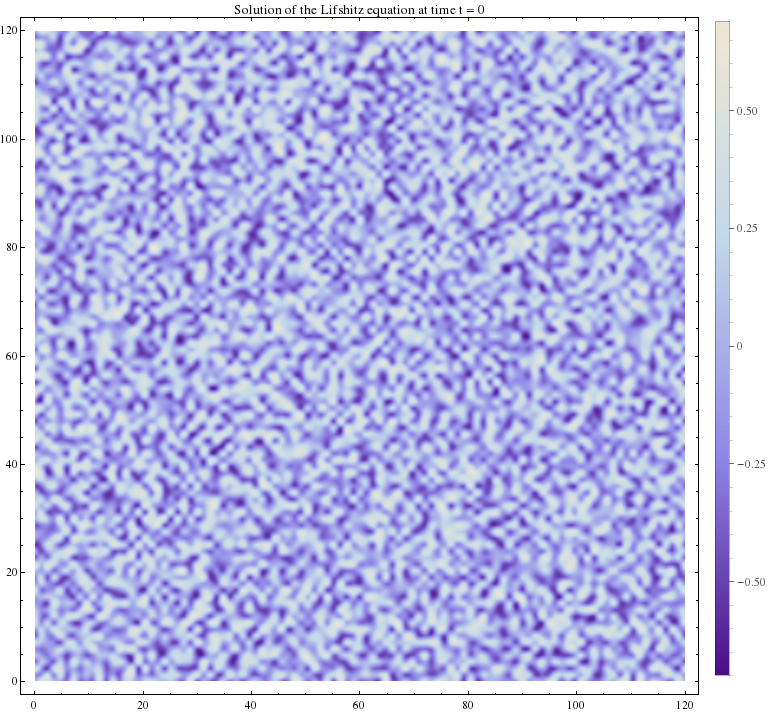
\includegraphics[scale=0.25]{img/sol_Lif_t0.png}\hfill%
\end{figure} 
}

\only<2>{
\begin{figure}[htp] 
\centering
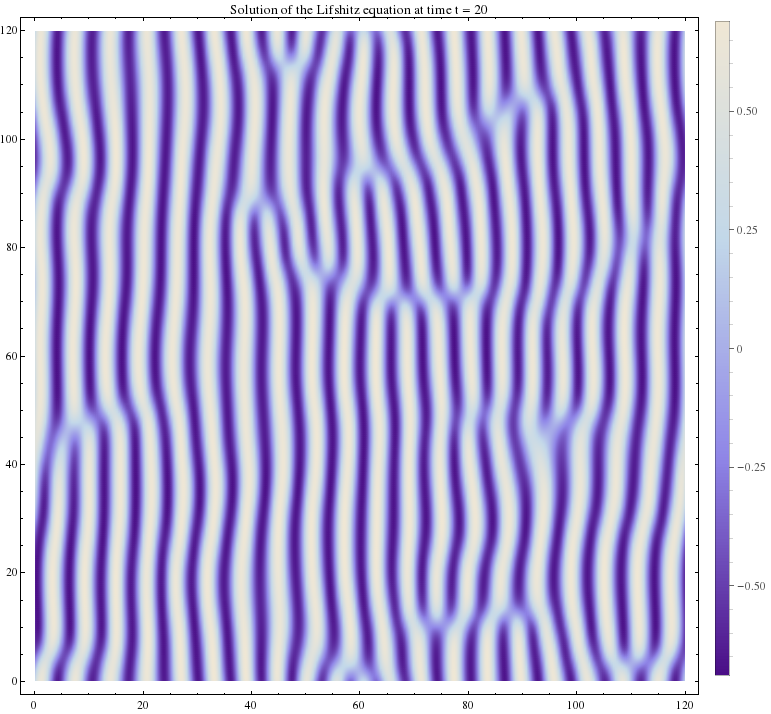
\includegraphics[scale=0.25]{img/sol_Lif_t20.png}\hfill%
\end{figure} 
}

\only<3>{
\begin{figure}[htp] 
\centering
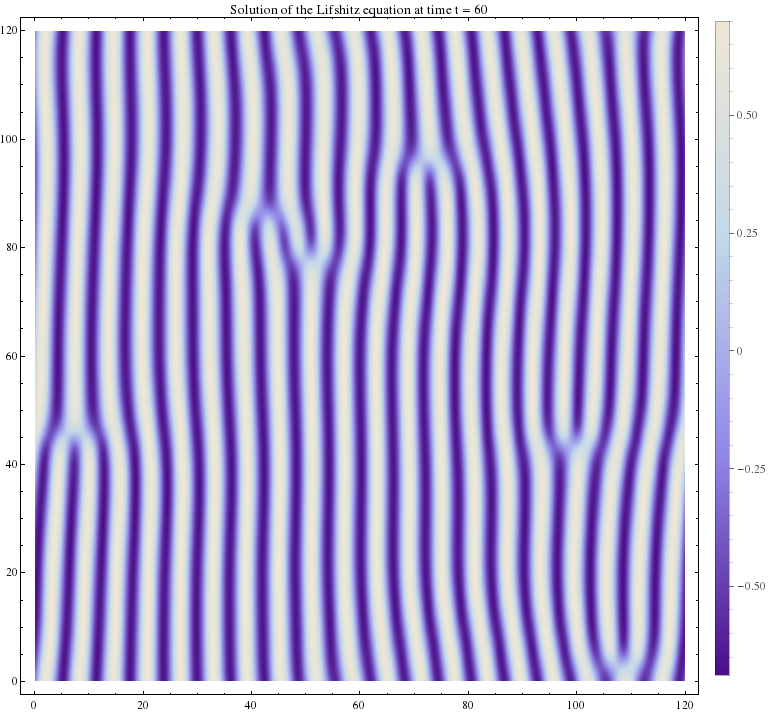
\includegraphics[scale=0.25]{img/sol_Lif_t60.png}\hfill%
\end{figure} 
}

\only<4>{
\begin{figure}[htp] 
\centering
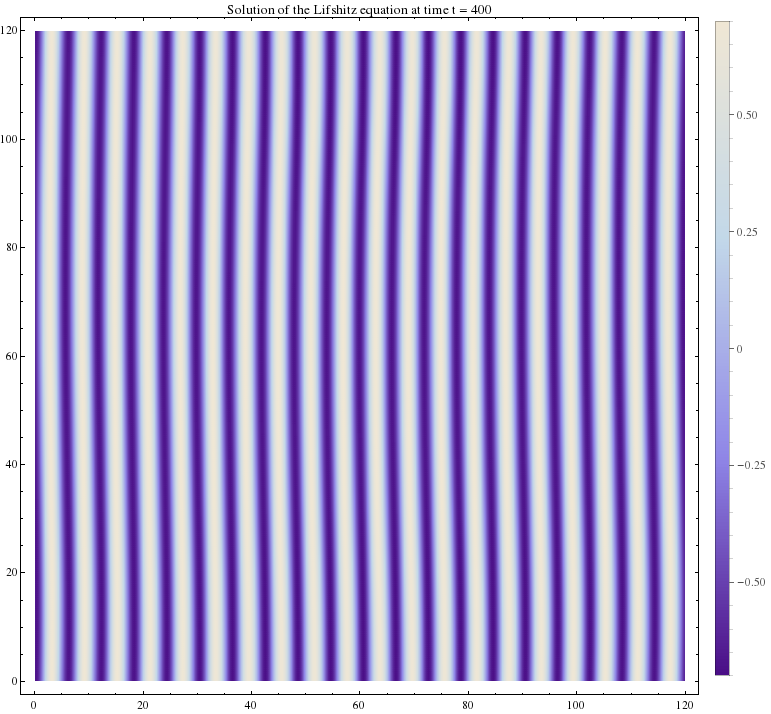
\includegraphics[scale=0.25]{img/sol_Lif_t400.png}\hfill%
\end{figure} 
}

\end{frame}

\begin{frame}

\begin{figure}[htp]
\centering
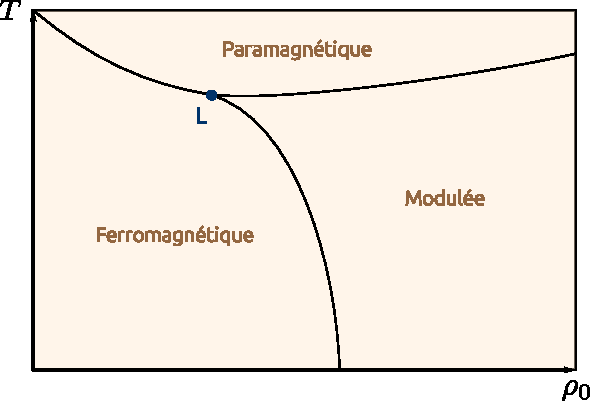
\includegraphics[scale=0.65]{img/phase_diagram.pdf}
\label{}
\end{figure}

\begin{block}{Hamiltonien de Lifshitz}
\centering
$ H[\boldsymbol{\phi}] = \int_x  \frac{1}{2}(\p{\perp} \boldsymbol{\phi})^2 + \frac{\rho_0}{2}(\p{\sslash} \boldsymbol{\phi})^2 + \frac{\sigma_0}{2} (\p{\sslash}^2 \boldsymbol{\phi})^2 + U(\rho) \text{,~} \rho \define \frac{\boldsymbol{\phi}^2}{2}$
\end{block}

\end{frame}

\section{Le groupe de renormalisation non perturbatif}
\subsection{L'idée de la renormalisation}
\begin{frame}

\only<1>{
\begin{figure}[htp]
\centering

\includegraphics[scale=0.35]{img/renorm_step0.pdf}
\label{}
\end{figure}
\[H[\phi(x_i)]\]
\[\phantom{\tilde{\phi}_B = \frac{1}{Sa} \sum_{i \in B} \phi_i}\]
}

\only<2>{
\begin{figure}[htp]
\centering
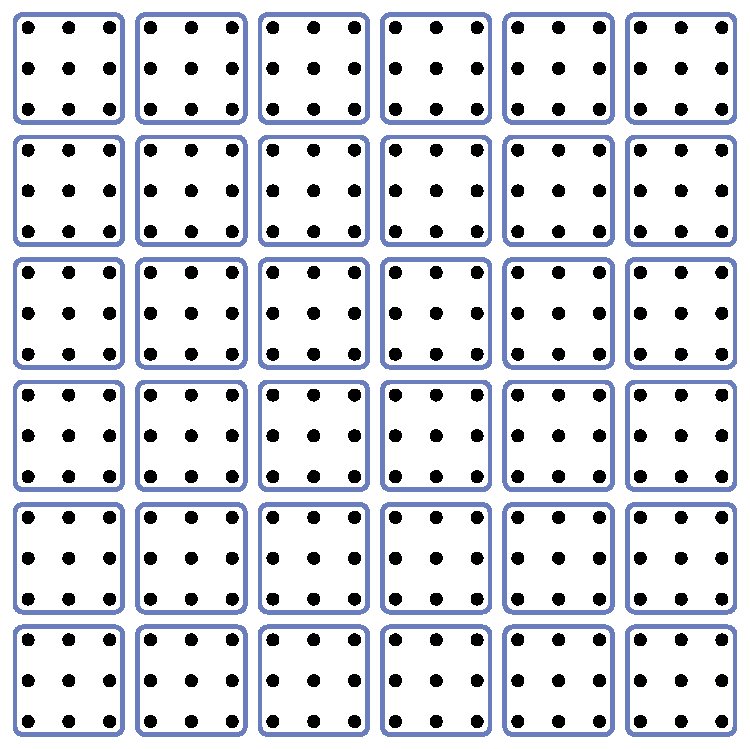
\includegraphics[scale=0.35]{img/renorm_step1.pdf}
\label{}
\end{figure}
\[H[\phi(x_i)]\]
\[\tilde{\phi}(x_b) = \frac{1}{Sa} \sum_{i \in b} \phi(x_i)\]
}

\only<3>{
\begin{figure}[htp]
\centering

\includegraphics[scale=0.35]{img/renorm_step2.pdf}
\label{}
\end{figure}
\[H[\phi(x_i)] \rightarrow \tilde{H}[\tilde{\phi}(x_b)]\]
\[\phantom{\tilde{\phi}_b = \frac{1}{Sa} \sum_{i \in b} \phi_i}\]
}

\only<4>{
\begin{figure}[htp]
\centering

\includegraphics[scale=0.35]{img/renorm_step3.pdf}
\label{}
\end{figure}
\[
 \left.\begin{aligned}
        x' = x/S \\
        \phi' = S^\Delta \phi
       \end{aligned}
 \right\}
  \rightarrow H_S[\phi'(x'_i)]
\]
Comparer $H$ et $H_S$ $\rightarrow$ renormalisation des constantes de couplage.
}
  
\end{frame}

\begin{frame}

\only<1>{
\begin{figure}[htp]
\centering
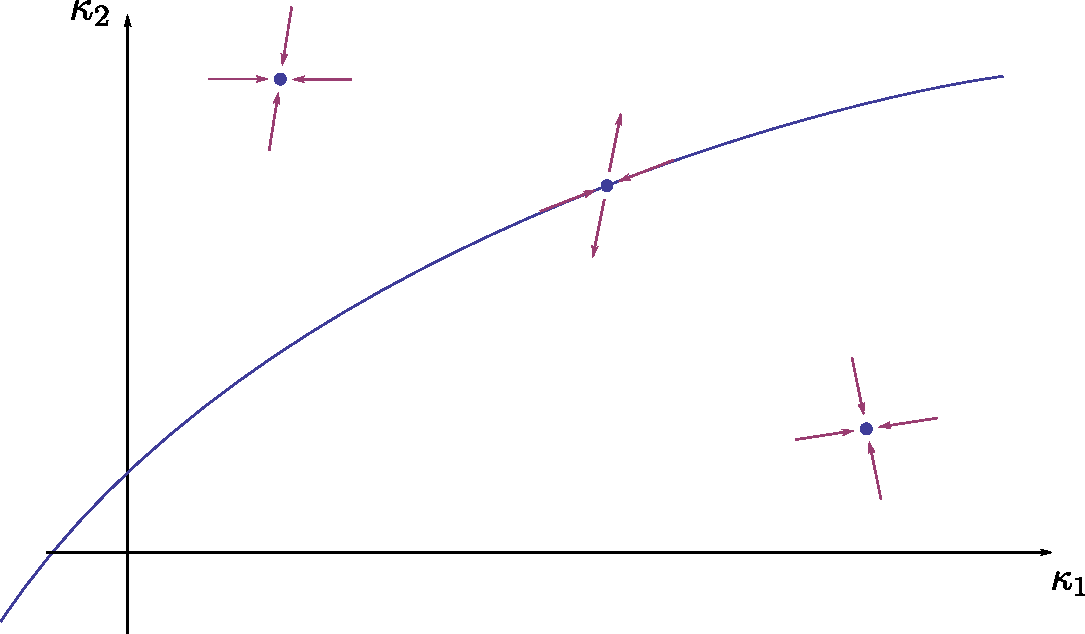
\includegraphics[scale=0.4]{img/flot.pdf}
\label{}
\end{figure}

\[
\text{Représentation schématique des flots dans l'espace des couplages.}
\]
}

\only<2>{
\begin{figure}[htp]
\centering
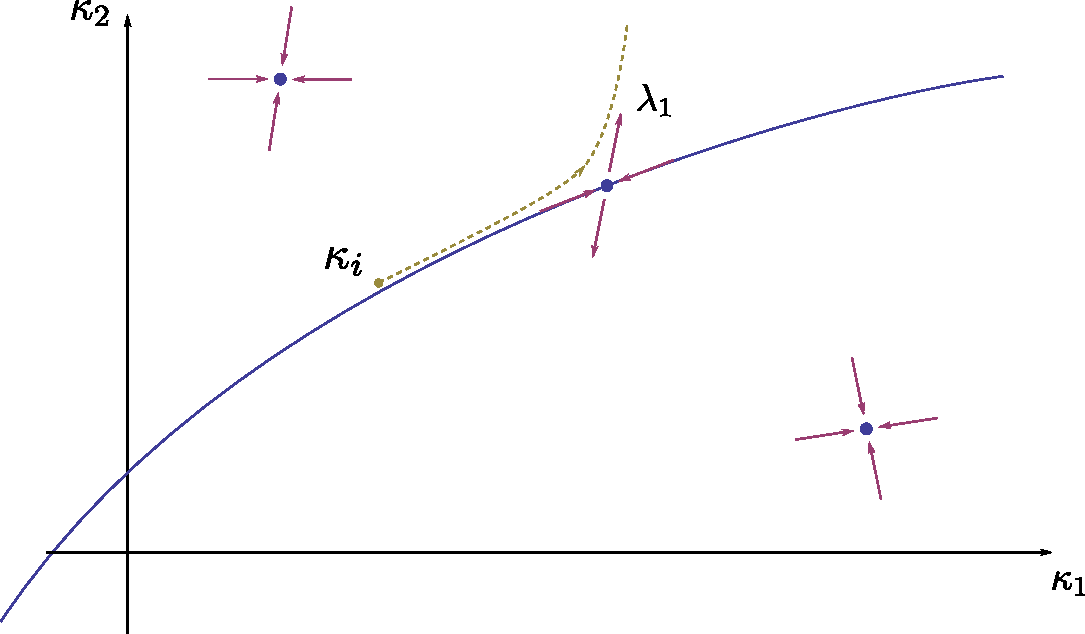
\includegraphics[scale=0.4]{img/flot_2.pdf}
\label{}
\end{figure}

\[
\xi \propto |T-T_c|^{-\nu} \text{,~} \nu = \frac{1}{\lambda_1}
\]
}

\end{frame}

\subsection{Application au modèle de Lifshitz en champ moyen}
\begin{frame}

\begin{figure}[htp]
\centering
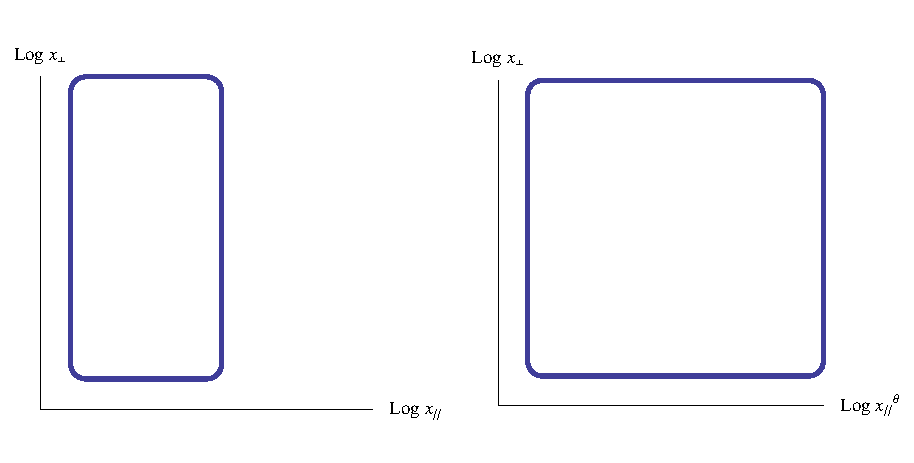
\includegraphics[scale=0.4]{img/blockspin_theta.pdf}
\label{}
\end{figure}
\begin{center}
Blocs de spin avant et après introduction de $\theta$.
\end{center}

\begin{block}{}
Directions inéquivalentes $\implies$ échelles inéquivalentes $S_\sslash$, $S_\perp$. \newline On introduit $\theta$ tel que $S_\sslash = S_\perp^\theta$. 
\end{block} 

\begin{block}{Résultats du champ moyen}
\centering
$\theta_\text{cm} = \frac{1}{2}$, $d_c^> = 4 + \frac{m}{2}$
\end{block}

\end{frame}

\subsection{Le groupe de normalisation non perturbatif}

\begin{frame}

\begin{columns}

\begin{column}{6cm}
\begin{figure}[htp]
\centering
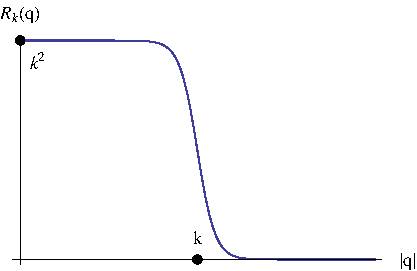
\includegraphics[scale=0.7]{img/regulator2.pdf}
\label{}
\end{figure}
\begin{center}
Dépendance en impulsion typique du régulateur $R_k(q)$.
\end{center}
\end{column}

\begin{column}{6cm}
\begin{figure}[htp]
\centering
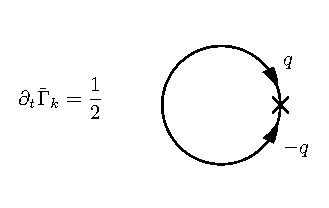
\includegraphics[scale=0.825]{img/dtgam.eps}
\label{}
\end{figure}
\[\p{t} \gam_k[\phi] = \frac{1}{2} \int_q \p{t}R_k(q)  G_k(q,-q)  \] 

\begin{figure}[htp]
\centering
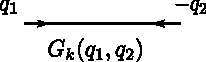
\includegraphics[scale=0.825]{img/propagateur.pdf}
\label{}
\end{figure}
\[G_k(q_1,q_2) =  \left( \Gamma^{(2)}_k + R_k \right)^{-1}_{q_1,q_2} \] 
\end{column}

\end{columns}

\end{frame}

\section{Le point critique de Lifshitz : méthodes et résultats}
\subsection{L'Ansatz pour l'action effective du modèle}
\begin{frame}

\begin{block}{Symétries $\implies$ forme générale de l'action effective de Lifshitz :}
$\Gamma_k[\phi] = \int_{x} U(\rho) + \left( \frac{1}{2} Z_\perp(\rho) (\partial_\perp \phi)^2 + \frac{1}{4} Y_\perp(\rho) (\partial_\perp \rho)^2 + ... \right) + \left( \frac{1}{2} \rho_0(\rho) (\partial_\sslash \phi)^2 + ... \right) + \left( \frac{1}{2} Z_\sslash(\rho) (\partial_\sslash^2 \phi)^2 + ... \right)$
\end{block}

Pour calculer les exposants critiques la structure impulsionnelle importe peu $\rightarrow$ simplifications.

\begin{block}{Forme définitive de l'Ansatz :}
$\Gamma_k[\phi_i] = \int_x  \frac{Z_\perp}{2} (\partial_\perp \phi)^2 + \frac{\rho_0}{2} (\partial_\sslash \phi)^2 + \frac{Z_\sslash}{2} (\partial_\sslash^2 \phi)^2 + U(\rho).$
\end{block}
\end{frame}

\subsection{Flots de renormalisation}
\begin{frame}

\begin{block}{Équations de flot du modèle}
\begin{itemize}
\item $\partial_t u_t(\rho) = -d_m u_t(\rho) + (\theta \eta_\sslash + d_m - 4 \theta) \rho u_t'(\rho)$ \\
\hfill $+~8 v_m v_{d-m} \left( l_0^{dm}\left(u_t'(\rho) + 2 \rho u_t''(\rho) \right) + (n-1)l_0^{dm}\left(u_t'(\rho)\right) \right)$

\item $\partial_t \rho_0 = -\theta \left(2-\eta_\sslash\right) \rho_0 - 64 \frac{ v_{d-m} v_m}{m} \rho u^{(2)}(\rho)^2 m_{1,2202} $

\item $\eta_\perp = 32 v_{d-m} v_m \rho u^{(2)}(\rho)^2$

\item $\eta_\sslash = \eta_\perp  \Big[ m_{1,3100} - \frac{1}{2} k_{1,2100}-\frac{2}{m}\left( 6 s_{1,4102}-6 v_{1,31002}+ w_{1,2102} \right)$ \\
\hfill$+~\frac{2}{m(m+2)}\big( 24 t_{1,5104} -36 z_{1,4104}+6 u_{1,3104} +8 y_{1,3104} - x_{1,2104} \big) \Big]$
\end{itemize}
\end{block}

Approximation du potentiel local : $\theta \simeq \theta_{\text{cm}} = \frac{1}{2}$, $\eta_{\sslash, \perp} \simeq \eta_{\text{cm}} = 0$.
\end{frame}

\subsection{Le potentiel au point de Lifshitz}

\begin{frame}
%\begin{block}{}
%$ 0 = -d_m u_t(\rho) + (\theta \eta_\sslash + d_m - 4 \theta) \rho u_t'(\rho)$ \\
%\hfill $+~8 v_m v_{d-m} \left( l_0^{dm}\left(u_t'(\rho) + 2 \rho u_t''(\rho) \right) + (n-1)l_0^{dm}\left(u_t'(\rho)\right) \right)$
%\end{block}
On a choisi de résoudre directement les équations de point fixe. 
\begin{block}{}
$0 = u(\rho) - a  \rho u'(\rho) + b(\rho_0) \left( \frac{1}{1 + \rho_0 + u'(\rho) + 2 \rho u''(\rho)} + \frac{n-1}{1+\rho_0+u'(\rho)} \right)$ \\
$u'(0) = \sigma$ \\
$u\phantom{'}(0) = n b(\rho_0)/(1+\sigma)$
\end{block}

\begin{block}{Stratégie de résolution}
\begin{itemize}
\item Commencer à $d=d_c^>$ ($\sigma^\text{Lif} = 0$, $\rho^\text{Lif}_{0} = 0$).
\item $d \rightarrow d - \delta d$. 
\item Trouver $\sigma^\text{Lif}$.
\item Trouver $\rho^\text{Lif}_{0}$.
\item Revenir à l'étape (2).
\end{itemize}
\end{block}

\end{frame}

\subsection{Les exposants critiques}

\begin{frame}
\only<1>{
\begin{figure}[htp] 
\centering
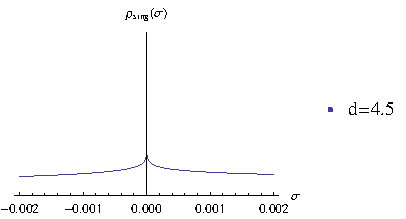
\includegraphics[scale=1.5]{img/emergence_lif_1.pdf}\hfill%
\end{figure} 
}

\only<2>{
\begin{figure}[htp] 
\centering
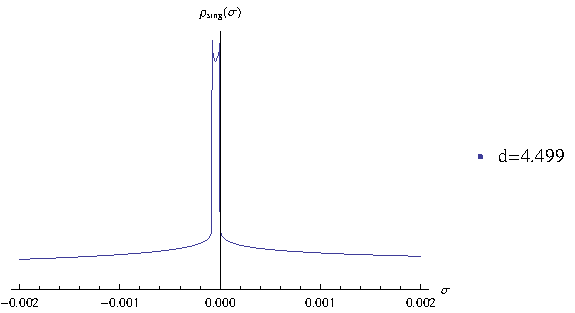
\includegraphics[scale=1.5]{img/emergence_lif_2.pdf}\hfill%
\end{figure} 
}

\only<3>{
\begin{figure}[htp] 
\centering
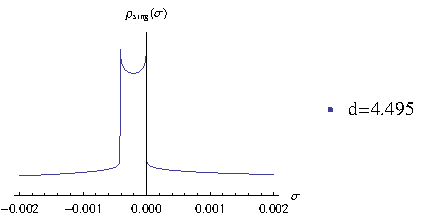
\includegraphics[scale=1.5]{img/emergence_lif_3.pdf}\hfill%
\end{figure} 
}

\only<4>{
\begin{figure}[htp] 
\centering
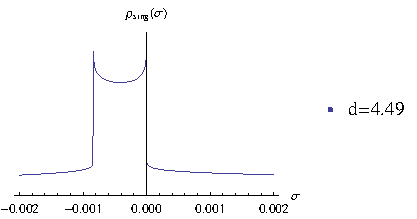
\includegraphics[scale=1.5]{img/emergence_lif_4.pdf}\hfill%
\end{figure} 
}

\only<5>{
\begin{figure}[htp] 
\centering
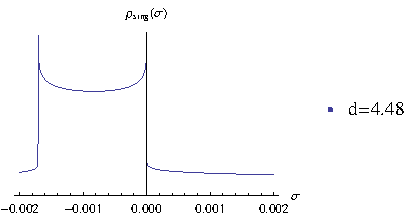
\includegraphics[scale=1.5]{img/emergence_lif_5.pdf}\hfill%
\end{figure} 
}
\end{frame}

\section{Conclusion}
\begin{frame}

\begin{itemize}
\item modélisation d'un phénomène mal compris : la ségrégation
\item relations entre physique, mathématiques et analyse numérique 
\item un domaine de la physique nouveau et en plein essor
\end{itemize}

\end{frame}

\end{document}